\documentclass[12pt,a4paper,ngerman]{article}
\usepackage{stylesheet}
\begin{document}
\TUHeader                          %  Bitte Ausfüllen!!!
%----------------------------
{Übung F: Übertragungsverhalten nachrichtentechnischer Systeme}                       %  Übungstitel
%----------------------------
{25.11.2014}                        %  Übungsdatum
%----------------------------
{05}                            %  Gruppen-Nr.
%----------------------------
{Thomas Neff}                   % Name des Protokollführers
%----------------------------
{
1.~Daniel Freßl, 1230028\\
2.~Thomas Neff, 1230319\\                    %  Übungsteilnehmer
3.~Thomas Pichler, 1230320 \\                   %  ...bei <4 Teilnehmer auskommentieren
4.~Martin Winter, 1130688\\
5.~Bernadette Schreyer, 1073076\\
}
%----------------------------
{Ao.Univ.-Prof. Dipl.-Ing. Dr. techn. Erich Leitgeb}
{Max Henkel}                          %  Betreuer
%----------------------------
{Graz}                              %  Ort der Protokollerstellung
{\today}                            %  Datum Protokollerstellung




\pagebreak
  
\tableofcontents
  
\pagebreak

%-------------------------------------------------------------------------------
%
% Beginn des Protokolls
%
%-------------------------------------------------------------------------------

\section{Übung 1}
\subsection{Aufgabenstellung}
In der ersten Übung galt es, die Spannungsverteilung über die ganze Messleitung bei kurzgeschlossenem Leitungsende aufzunehmen. Diese gemessene Spannungsverteilung ist graphisch in Prozenten vom Maximalwert darzustellen, im gleichen Diagramm ist die ideale berechnete Spannungsverteilung bei Kurzschluss einzuzeichnen. \\
Weiters ist die Ersatzimpedanz für den Kurzschluss und die Offset-Länge zum Kurzschluss zu ermitteln und im Smith-Diagramm einzuzeichnen und die Betriebsfrequenz des Oszillators zu berechnen. \\
Für den zweiten Teil der ersten Übung wird die Messleitung als ideal (verlustlos) angenommen, die Spannung war möglichst nahe an der Last abzugreifen, um diese Voraussetzung so gut als möglich zu erfüllen. Dabei waren zusätzlich die Ersatzimpedanzen für das offene Leitungsende und den handelsüblichen $50\Omega$ Abschluss zu berechnen und im Smith-Diagramm einzuzeichnen. Abschließend sollte die Impedanz des Dämpfungsgliedes in Serie mit dem Kurzschluss und die Dämpfung aus dem Betrag des Reflexionsfaktors bestimmt werden. 
\subsection{Schaltung}
\begin{figure}[h!]
\centering

\includegraphics[scale=1]{figures/schaltung.png}
\caption{Blockschaltbild der Messschaltung}
\end{figure}
\pagebreak
 
\subsection{Tabellen}
\begin{table}[h!]
  \begin{center}
    \begin{tabular}{| c | c |}
    \hline
    $z$  & $\frac{|U_z|}{|U_{max}|}$   \\ \hline \hline
    $-5$ & $0.98$ \\ \hline
    $-5.5$ & $1$ \\ \hline
    $-6$ & $0.91$ \\ \hline
    $-6.5$ & $0.72$ \\ \hline
    $-7$ & $0.48$ \\ \hline
    $-7.5$ & $0.185$ \\ \hline
    $-8$ & $0.091$ \\ \hline
    $-8.5$ & $0.37$ \\ \hline
    $-9$ & $0.63$ \\ \hline
    $-9.5$ & $0.84$ \\ \hline
    $-10$ & $0.975$ \\ \hline
    $-10.5$ & $1$ \\ \hline
    $-11$ & $0.91$ \\ \hline
    $-11.5$ & $0.72$ \\ \hline
    $-12$ & $0.46$ \\ \hline
    \end{tabular}
  \end{center}
  \caption{Aufnahme der Spannungsverteilung}
\end{table}
\subsection{Formeln}
Für den idealen Spannungsverlauf entlang der Leitung bei kurzgeschlossenem Leitungsende erhält man
\begin{equation}
\frac{|U_z|}{|U_{max}|} = \left|sin\left(\frac{2\pi}{\lambda} \cdot z\right)\right|
\end{equation}
$U_{max}$ wird auf 1 normiert, dies ermöglicht
\begin{equation}
m = \frac{|U_{min}|}{|U_{max}|} = \frac{|U_{min}|}{1} \quad \Rightarrow \quad	 U_{min} = m \quad m \text{ ... Stehwellenverhältnis}
\end{equation}
Für den Reflexionsfaktor $\rho_0$ gilt
\begin{equation}
|\rho_0| = \frac{1-m}{1+m}
\end{equation}
Die Wellenlänge $\lambda$ ergibt sich zu
\begin{equation}
\lambda_{ideal} = \frac{c}{\nu} = \frac{3 \cdot 10^8 m/s}{3 \cdot 10^9 1/s} = 0.1m
\end{equation}
\subsection{Berechnungsbeispiele}
\subsubsection{Kurzschluss}
Es gilt die Ersatzimpedanz für den Kurzschluss zu bestimmen, dabei wurde ein Minimum bestimmt bei $z = -7.8cm$ bei einem proportionalen Wert von $U_{min}=m=0.012$. Aufgrund der periodischen Struktur($\frac{\lambda}{2} = 0.05m$) lässt sich das erste Minimum bei $z=-2.8cm$ berechnen, was gleich $l_0$ ist. Dies normiert ergibt sich zu
\begin{equation}
\frac{l_0}{\lambda} = \frac{2.8 \cdot 10^{-2}m}{0.1m} = 0.28
\end{equation}
Der Reflexionsfaktor ergibt sich zu
\begin{equation}
|\rho_0|_{KS} = \frac{1-m}{1+m} = \frac{1-0.012}{1+0.012} = 0.976
\end{equation}
Durch graphische Darstellung im Smith-Diagramm ergibt sich für die Ersatzimpedanz
\begin{equation}
\underline{Z}_{L,N} = 0.2 + j5.3 \quad \Rightarrow \quad \underline{Z}_L = \frac{\underline{Z}_{L,N}}{\underline{Z}_W} = 10 + j265 \ \Omega
\end{equation}
Die reale Betriebsfrequenz des Oszillators errechnet sich zu
\begin{equation}
c = \lambda \cdot \nu \quad \Rightarrow \quad \nu_{Oszillator} = \frac{c}{\lambda} = \frac{3 \cdot 10^8m/s}{0.1m} = 3\ GHz
\end{equation}
\subsubsection{Leerlauf}
Es gilt die Ersatzimpedanz für den Leerlauf zu bestimmen, dabei wurde ein Minimum bestimmt bei $z = -10.27$ von einem proportionalen Wert von $U_{min}=m=0.036$. Aufgrund der periodischen Struktur lässt sich das erste Minimum bei $z=-0.27$ berechnen, was gleich $l_0$ ist. Dies normiert ergibt sich zu
\begin{equation}
\frac{l_0}{\lambda} = \frac{0.27 \cdot 10^{-2}m}{0.1m} = 0.027
\end{equation}
Der Reflexionsfaktor ergibt sich zu
\begin{equation}
|\rho_0|_{LL} = \frac{1-m}{1+m} = \frac{1-0.036}{1+0.036} = 0.9305
\end{equation}
Durch graphische Darstellung im Smith-Diagramm ergibt sich für die Ersatzimpedanz
\begin{equation}
\underline{Z}_{L,N} = 0.038 - j0.17 \quad \Rightarrow \quad \underline{Z}_L = \frac{\underline{Z}_{L,N}}{\underline{Z}_W} = 1.9 - j8.5 \ \Omega
\end{equation}
\pagebreak

\subsubsection{$50\Omega$ Abschluss}
Es gilt die Ersatzimpedanz für den $50\Omega$ Abschluss zu bestimmen, dabei wurde ein Minimum bestimmt bei $z = -10.17$ von einem proportionalen Wert von $U_{min}=m=0.86$. Aufgrund der periodischen Struktur lässt sich das erste Minimum bei $z=-0.17$ berechnen, was gleich $l_0$ ist. Dies normiert ergibt sich zu
\begin{equation}
\frac{l_0}{\lambda} = \frac{0.17 \cdot 10^{-2}m}{0.1m} = 0.017
\end{equation}
Der Reflexionsfaktor ergibt sich zu
\begin{equation}
|\rho_0|_{50} = \frac{1-m}{1+m} = \frac{1-0.86}{1+0.86} = 0.0753
\end{equation}
Durch graphische Darstellung im Smith-Diagramm ergibt sich für die Ersatzimpedanz
\begin{equation}
\underline{Z}_{L,N} = 0.87 - j 0.03 \quad \Rightarrow \quad \underline{Z}_L = \frac{\underline{Z}_{L,N}}{\underline{Z}_W} = 43.5 - j1.5 \ \Omega
\end{equation}

\subsubsection{Kurzschluss mit Abschwächer}
Es gilt die Ersatzimpedanz für den Kurzschluss mit Abschwächer zu bestimmen, dabei wurde ein Minimum bestimmt bei $z = -10.02$ von einem proportionalen Wert von $U_{min}=m=0.71$. Aufgrund der periodischen Struktur lässt sich das erste Minimum bei $z=-0.02$ berechnen, was gleich $l_0$ ist. Dies normiert ergibt sich zu
\begin{equation}
\frac{l_0}{\lambda} = \frac{0.02 \cdot 10^{-2}m}{0.1m} = 0.002
\end{equation}
Der Reflexionsfaktor ergibt sich zu
\begin{equation}
|\rho_0|_{\text{KS,Abschwächer}} = \frac{1-m}{1+m} = \frac{1-0.71}{1+0.71} = 0.1696
\end{equation}
Durch graphische Darstellung im Smith-Diagramm ergibt sich für die Ersatzimpedanz
\begin{equation}
\underline{Z}_{L,N} = 0.7 - j0.01 \quad \Rightarrow \quad \underline{Z}_L = \frac{\underline{Z}_{L,N}}{\underline{Z}_W} = 35-j0.5 \ \Omega
\end{equation}
Die Dämpfung lässt sich folgendermaßen berechnen
\begin{equation}
d[dB] = \frac{1}{2} \ 20 \ log\left( \frac{|\underline{\rho}_0|_{KS}}{|\underline{\rho}_0|_{\text{KS,Abschwächer}}}\right) = \frac{1}{2}\ 20\ log\left( \frac{0.976}{0.1696}\right)= 7.6002 \ dB
\end{equation}




\pagebreak
\subsection{Diagramme}


\begin{figure}[h!]
\centering
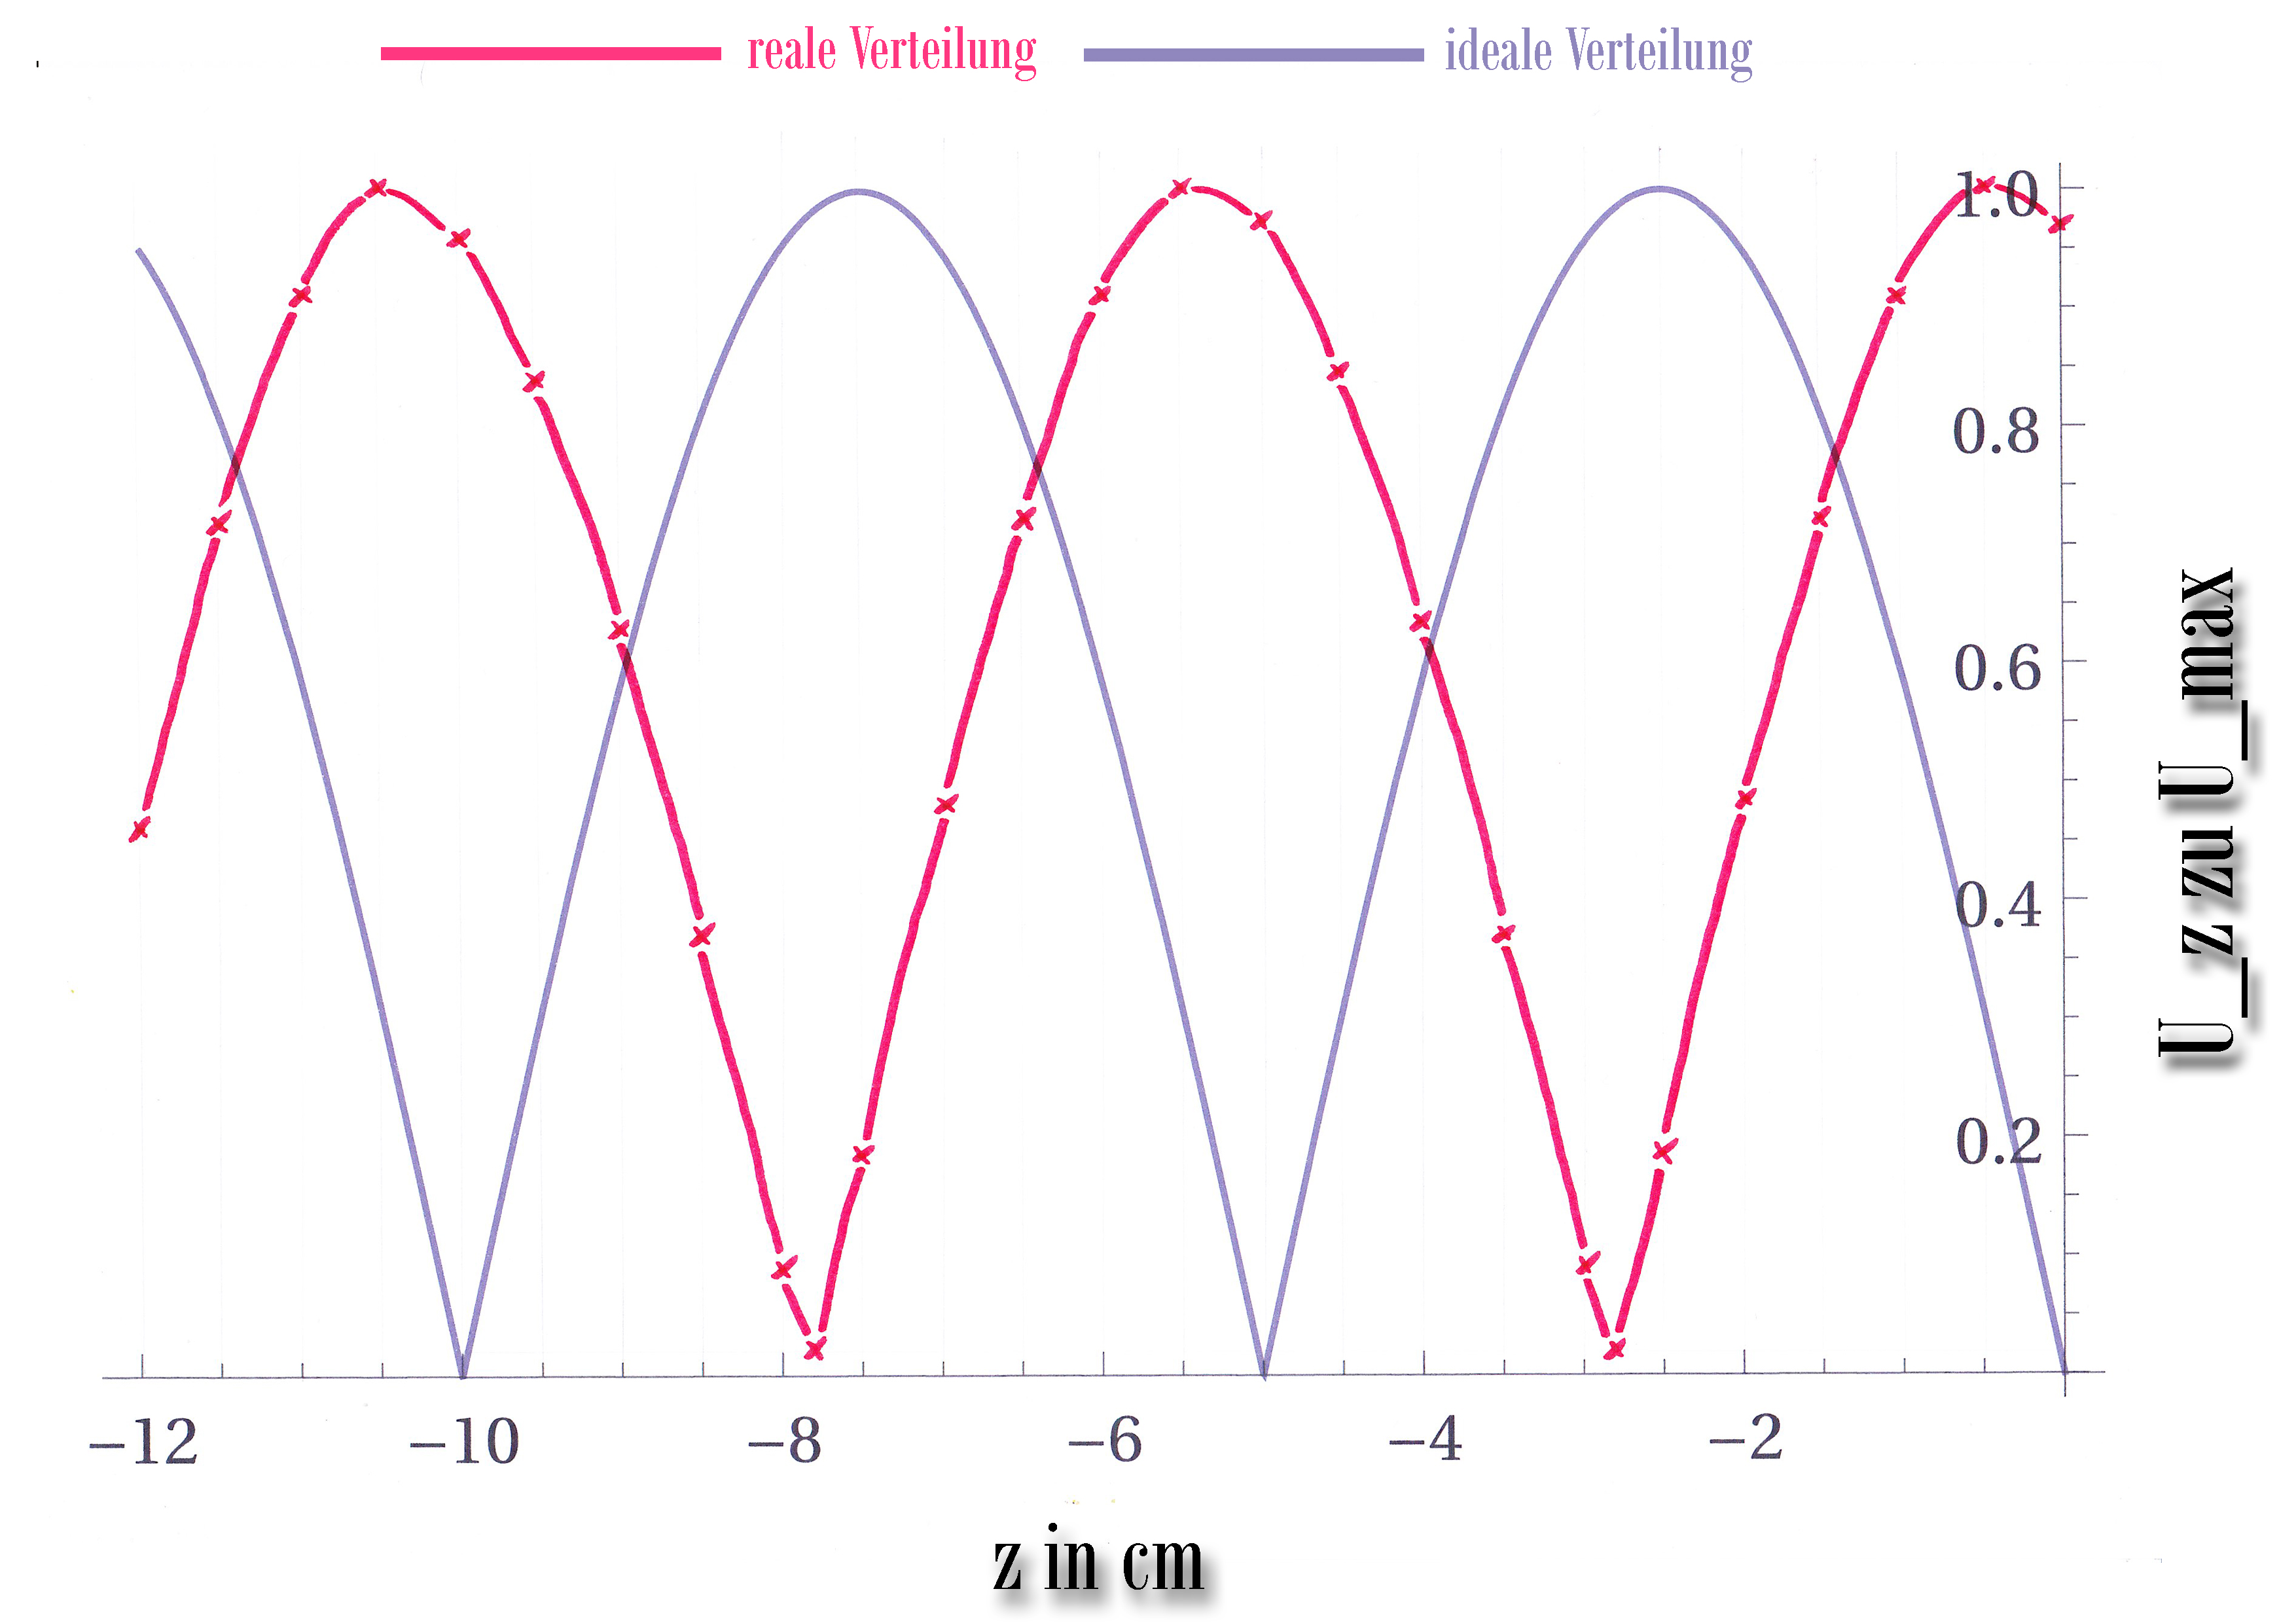
\includegraphics[scale=0.13]{figures/graph.jpg}
\caption{Graph über die Spannungsverteilung im Verhältnis zum Maximalwerts}
\end{figure}

\pagebreak
\begin{figure}[h!]
\centering
\includegraphics[scale=0.085]{figures/scan_uebung1.jpg} 
\caption{Smith-Diagramm zu den 4 Aufgabenstellungen}
\end{figure}

\subsection{Diskussion}
Um den Spannungsverlauf aufnehmen zu können, wurde $U_{max}$ auf 1 normiert, damit erhielt man die Äquivalenz von $U_{min}$ und $m$ und konnte den Spannungsverlauf $\frac{U_Z}{U_{max}} = \frac{U_Z}{1} = U_Z$ messen. Man konnte beim Kurzschluss sehr gut die Abweichung vom idealen Verhalten erkennen, bei den verwendeten hohen Frequenzen treten zusätzliche Effekte auf, die zu Abweichungen von der idealen Kennlinie führen, durch parasitäre Kopplungen erhält man so ein induktives Verhalten, da der Kurzschluss bei sehr hohen Frequenzen als einfache Leitung selbst als Induktivität wirkt. \\
Beim Leerlauf konnte man ebenfalls sehr gut die Abweichung vom idealen Verhalten erkennen, verursacht durch hohe parasitäre Kapazitäten, die offenen Leitungsenden wirken wie Kondensatoren. \\
Bei dem $50 \Omega$ Abschluss konnte ein recht gutes Verhalten gemessen werden, die Abweichungen vom idealen Verhalten waren bei weitem nicht so gravierend zu sehen wie bei Kurzschluss und Leerlauf. \\
Bei der letzten Unterübung wurde noch ein Dämpfungsglied in Serie zum Kurzschluss eingebaut, dadurch wurde auch der Reflexionsfaktor entsprechend gedämpft.
Durch die endliche Ablesegenauigkeit ergab sich die gemessene Oszillatorfrequenz zufälligerweise genau zu der idealen Oszillatorfrequenz, dies lässt sich durch die beschränkte Genauigkeit beim Ablesen erklären. 
\pagebreak









\section{Übung 2}
\subsection{Aufgabenstellung}
Ziel dieser Übung war es, mit der \textbf{AWR-Software} gegebene Aufgaben zu simulieren und die erhalten Ergebnisse ebenfalls noch in Papierform mittels Smith-Diagrammen zu verifizieren. Die Schaltung wird dabei mit einer Frequenz von 3 Ghz betrieben und es waren 4 verschiedene Unteraufgaben zu bewältigen. 
\subsection{Schaltung}
\subsubsection{Schaltung zu Aufgabe 1}
\begin{figure}[h!]
\centering
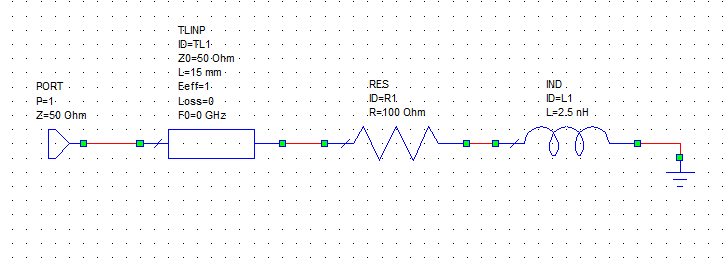
\includegraphics[scale=0.7]{figures/Aufgabe1_sch.png} 
\caption{Schaltung 1}
\end{figure}
\subsubsection{Schaltung zu Aufgabe 2}
\begin{figure}[h!]
\centering
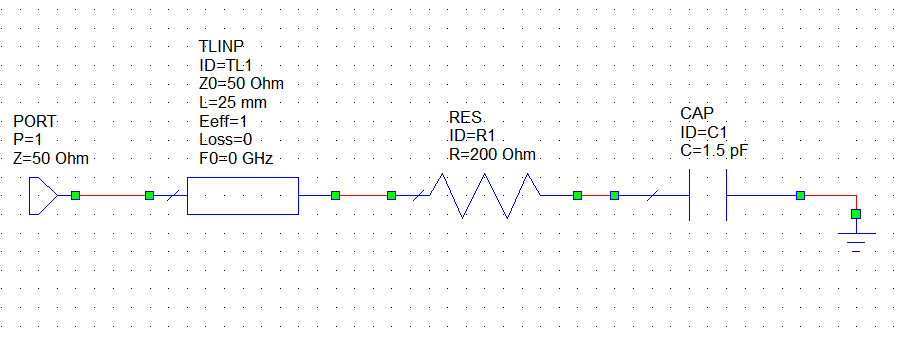
\includegraphics[scale=0.7]{figures/Aufgabe2_sch.png} 
\caption{Schaltung 2}
\end{figure}
\pagebreak
\subsubsection{Schaltung zu Aufgabe 3}
\begin{figure}[h!]
\centering
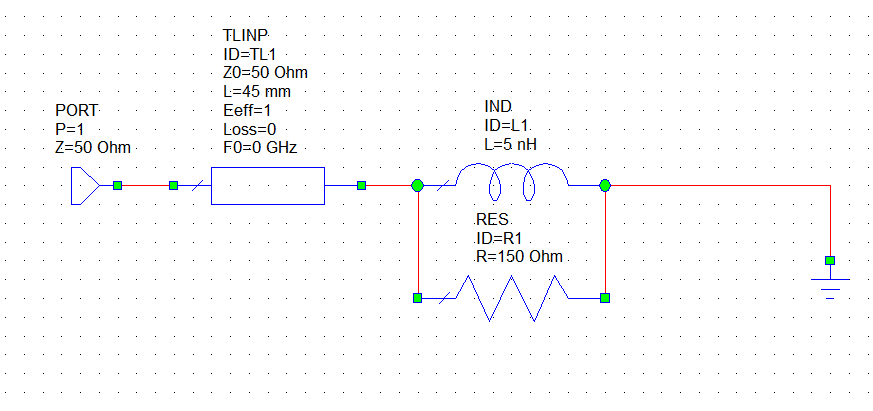
\includegraphics[scale=0.7]{figures/Aufgabe3_sch.png} 
\caption{Schaltung 3}
\end{figure}
\subsubsection{Schaltung zu Aufgabe 4}
\begin{figure}[h!]
\centering
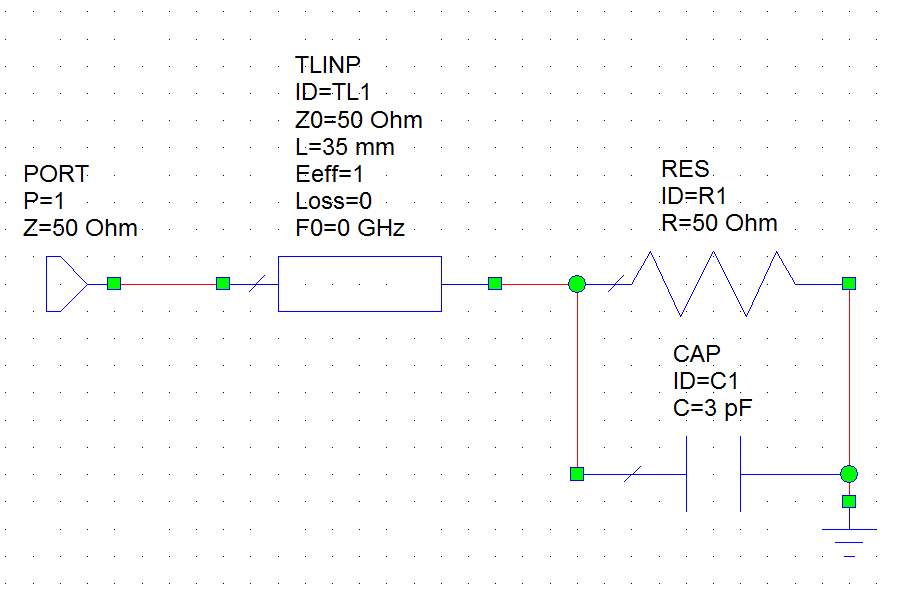
\includegraphics[scale=0.6]{figures/Aufgabe4_sch.png} 
\caption{Schaltung 4}
\end{figure}


\pagebreak

\subsection{Formeln}
Die Winkelgeschwindigkeit $\omega$ ergibt sich zu
\begin{equation}
\omega = 2 \pi \cdot \nu = 2 \pi \cdot 3 \cdot 10^9 = 1.88496 \cdot 10^{10} rad/s
\end{equation}
Die Wellenlänge $\lambda$ errechnet sich folgendermaßen
\begin{equation}
\lambda = \frac{c}{\nu} = \frac{3 \cdot 10^8\frac{m}{s}}{3 \cdot 10^9 \frac{1}{s}} = 0.1m
\end{equation}
\subsection{Berechnungsbeispiele}
Man berechnet zuerst $\underline{Z}_L$, normiert diesen und dreht ihn um $l_0$ Richtung Generator, entnormiert den abgelesenen Wert um $\underline{Z}_{in}$ zu erhalten.
\subsubsection{Aufgabe 1}
\begin{gather}
\underline{Z}_L = r + j\omega L = 100 +j1.88496 \cdot 10^{10} \cdot 2.5 \cdot 10^{-9} = 100 +j47.124 \Omega \\
\underline{Z}_{L,N} = \frac{\underline{Z}_L}{\underline{Z}_W} = \frac{100+j47.124}{50} = 2 + j0.9425 \\
l_0 = 0.015m \\
l_{0,N} = \frac{l_0}{\lambda} = \frac{0.015}{0.1} = 0.15 \\
\text{Drehen um }l_{0,N} \text{ Richtung Generator}\Rightarrow \quad \underline{Z}_{in,N} = 0.77 -j0.82 \\
\underline{Z}_{in} = \underline{Z}_{in,N} \cdot \underline{Z}_W = 38.5 - j41 \Omega
\end{gather}

\subsubsection{Aufgabe 2}
\begin{gather}
\underline{Z}_L = r + \frac{1}{j\omega C} = 200 +\frac{1}{j 1.8849 \cdot 10^9 \cdot 1.5 \cdot 10^{-12}}	 = 200 -j35.3678 \Omega\\
\underline{Z}_{L,N} = \frac{\underline{Z}_L}{\underline{Z}_W} = \frac{200 -j35.3678}{50} = 4-j0.707 \\
l_0 = 0.025m \\
l_{0,N} = \frac{l_0}{\lambda} = \frac{0.025}{0.1} = 0.25 \\
\text{Drehen um }l_{0,N} \text{ Richtung Generator}\Rightarrow \quad \underline{Z}_{in,N} = 0.24 + j0.045 \\
\underline{Z}_{in} = \underline{Z}_{in,N} \cdot \underline{Z}_W = 12+j2.25 \Omega
\end{gather}

\pagebreak

\subsubsection{Aufgabe 3}
\begin{gather}
\underline{Z}_L = \frac{j\omega L \cdot R}{j\omega L + R} \\
\omega L = 2 \pi \nu L = 2 \pi \cdot 3 \cdot 10^9 \cdot 5 \cdot 10^{-9} = 94.24 \Omega\\
\Rightarrow \quad \frac{j 94.24 \cdot 150}{j94.24 +150} = \frac{j14136}{j94.24 + 150} \quad \Rightarrow \quad \underline{Z}_{L} = 42.45 + j67.5698 \Omega \\
\underline{Z}_{L,N} = \frac{\underline{Z}_L}{\underline{Z}_W} = \frac{42.45 + j67.5698}{50} = 0.849 + j1.351  \\
l_0 = 0.045m \\
l_{0,N} = \frac{l_0}{\lambda} = \frac{0.045}{0.1} = 0.45 \\
\text{Drehen um }l_{0,N} \text{ Richtung Generator}\Rightarrow \quad \underline{Z}_{in,N} = 0.8+j0.44 \\
\underline{Z}_{in} = \underline{Z}_{in,N} \cdot \underline{Z}_W = 40 + j22 \Omega
\end{gather}

\subsubsection{Aufgabe 4}
\begin{gather}
\underline{Z}_L = \frac{\frac{1}{j \omega C} \cdot R}{\frac{1}{j \omega C} + R} = \frac{R \cdot \frac{1}{j \omega C}}{R-j\frac{1}{\omega C}} \cdot \frac{R+j\frac{1}{\omega C}}{R+j\frac{1}{\omega C}} = \frac{\frac{R}{\j \omega C}(R+j\frac{1}{\omega C})}{R^2 + (\frac{1}{\omega C})^2} =\\
= \frac{\frac{R}{(\omega C)^2} -j\frac{R^2}{\omega C}}{R^2 + (\frac{1}{\omega C})^2} = \frac{15635.985 -j 44209.706}{2500 + 312.719} = 5.559 - j15.7178\Omega\\
\underline{Z}_{L,N} = \frac{\underline{Z}_L}{\underline{Z}_W} = \frac{5.559 - j15.7178}{50} = 0.11118 -j0.3144  \\
l_0 = 0.035m \\
l_{0,N} = \frac{l_0}{\lambda} = \frac{0.035}{0.1} = 0.35 \\
\text{Drehen um }l_{0,N} \text{ Richtung Generator}\Rightarrow \quad \underline{Z}_{in,N} = 0.9 -j2.7 \\
\underline{Z}_{in} = \underline{Z}_{in,N} \cdot \underline{Z}_W = 45-j135 \Omega
\end{gather}



\pagebreak
\subsection{Diagramme}
\subsubsection{Smith-Diagramm zu Aufgabe 1}
\begin{figure}[h!]
\centering
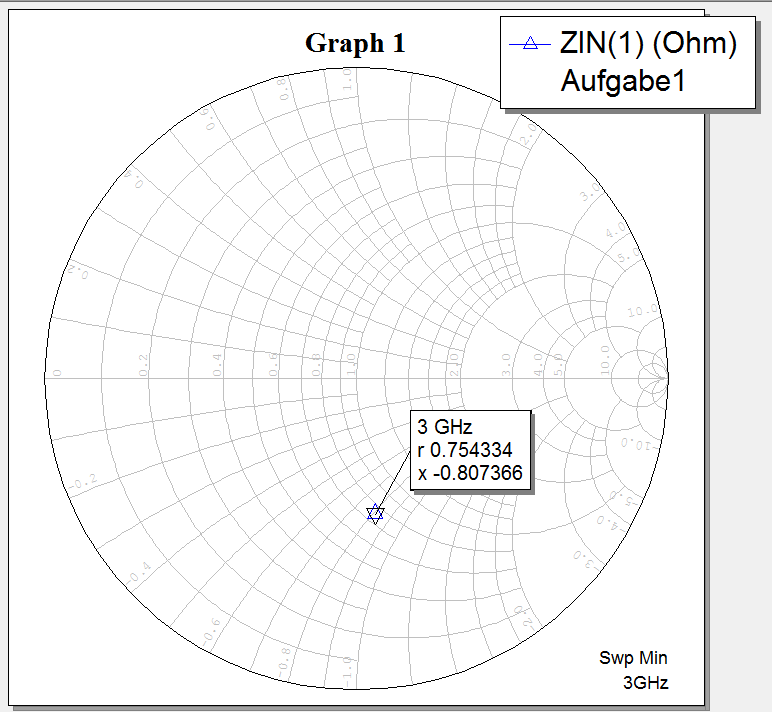
\includegraphics[scale=0.7]{figures/Aufgabe1_dia.png} 

\end{figure}

\pagebreak
\begin{figure}[h!]
\centering
\includegraphics[scale=0.085]{figures/scan_aufgabe1.jpg} 
\caption{Smith-Diagramm zu Aufgabe 1}
\end{figure}
\pagebreak
\subsubsection{Smith-Diagramm zu Aufgabe 2}
\begin{figure}[h!]
\centering
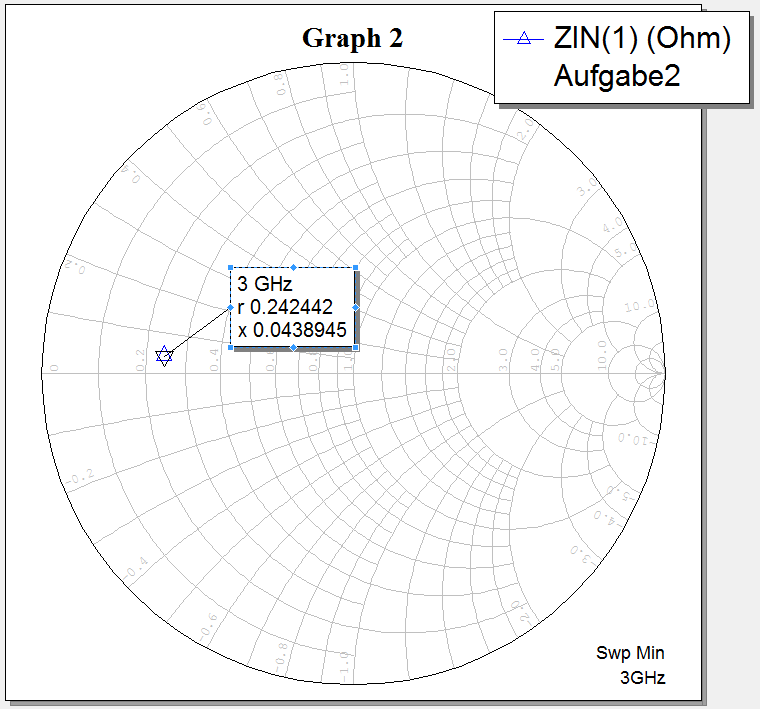
\includegraphics[scale=0.7]{figures/Aufgabe2_dia.png} 

\end{figure}
\pagebreak
\pagebreak
\begin{figure}[h!]
\centering
\includegraphics[scale=0.085]{figures/scan_aufgabe2.jpg} 
\caption{Smith-Diagramm zu Aufgabe 2}
\end{figure}
\subsubsection{Smith-Diagramm zu Aufgabe 3}
\begin{figure}[h!]
\centering
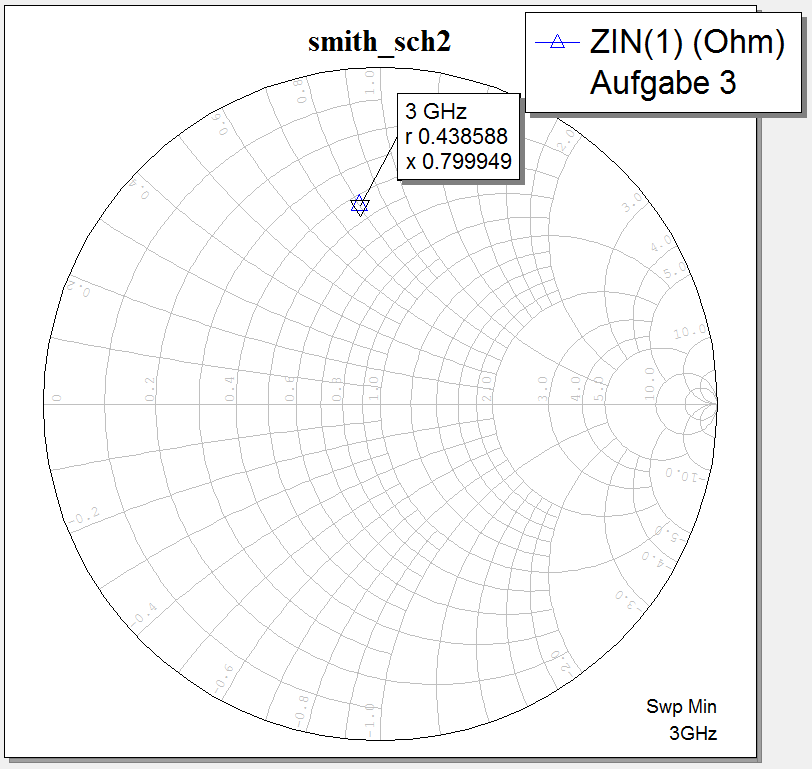
\includegraphics[scale=0.7]{figures/Aufgabe3_dia.png} 

\end{figure}
\pagebreak
\begin{figure}[h!]
\centering
\includegraphics[scale=0.085]{figures/scan_aufgabe3.jpg} 
\caption{Smith-Diagramm zu Aufgabe 3}
\end{figure}
\pagebreak
\subsubsection{Smith-Diagramm zu Aufgabe 4}
\begin{figure}[h!]
\centering
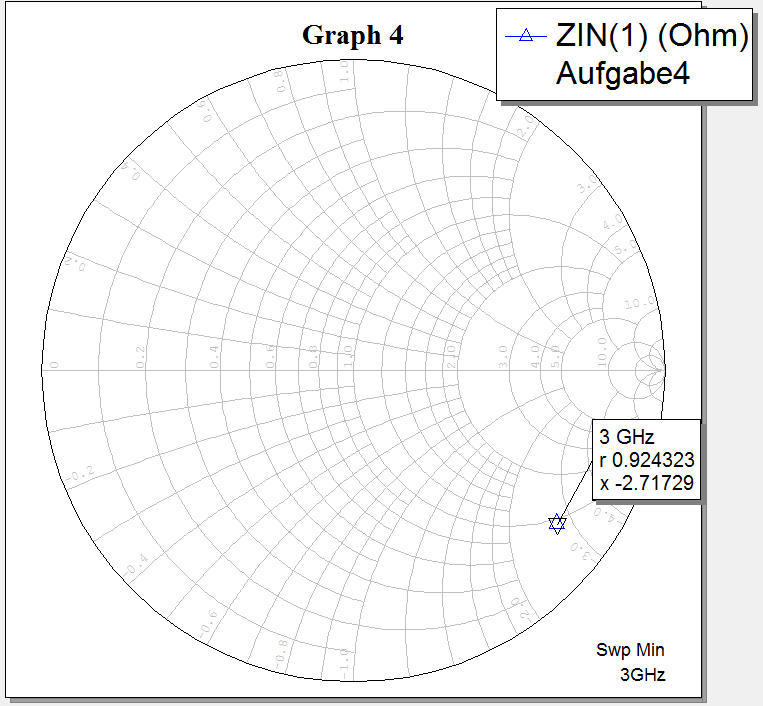
\includegraphics[scale=0.7]{figures/Aufgabe4_dia.png} 
\end{figure}
\pagebreak
\begin{figure}[h!]
\centering
\includegraphics[scale=0.085]{figures/scan_aufgabe4.jpg} 
\caption{Smith-Diagramm zu Aufgabe 4}
\end{figure}

\subsection{Diskussion}
Um die Eingangsimpedanz der Leitung zu bestimmen, wurde die Lastimpedanz berechnet, anschließend normiert und ins Smith-Diagramm eingetragen. Dann wurde der Punkt um die normierte Leitungslänge in Richtung Generator gedreht, abgelesen und entnormiert. \\
Bei allen vier Beispielen ergab die Simulation sowie unsere Berechnungsbeispiele die selben Ergebnisse. 











 



   
\end{document}